\section{Étude métrologique}\label{sec:etude-metrologique}
   Maintenant que les différentes données extraites des acquisitions peuvent être visualisées, il convient de mener une étude métrologique des mesures effectuées par les deux récepteurs GNSS afin de déterminer entre autres leur précision.

   \subsection{Cadre de l'étude}\label{subsec:cadre-de-l'etude}
      Pour réaliser cette étude, il est tout naturellement nécessaire de prendre des mesures expérimentales.

      Ainsi, nous avons placé successivement les deux récepteurs GNSS à un emplacement défini du campus, dont les coordonnées sont connues avec une très grande précision.
      Ce qui permettra de comparer les mesures expérimentales au point considéré comme \og exact \fg{}, donnant une information sur la précision du positionnement des récepteurs.

      \begin{figure}[h]
          \centering
          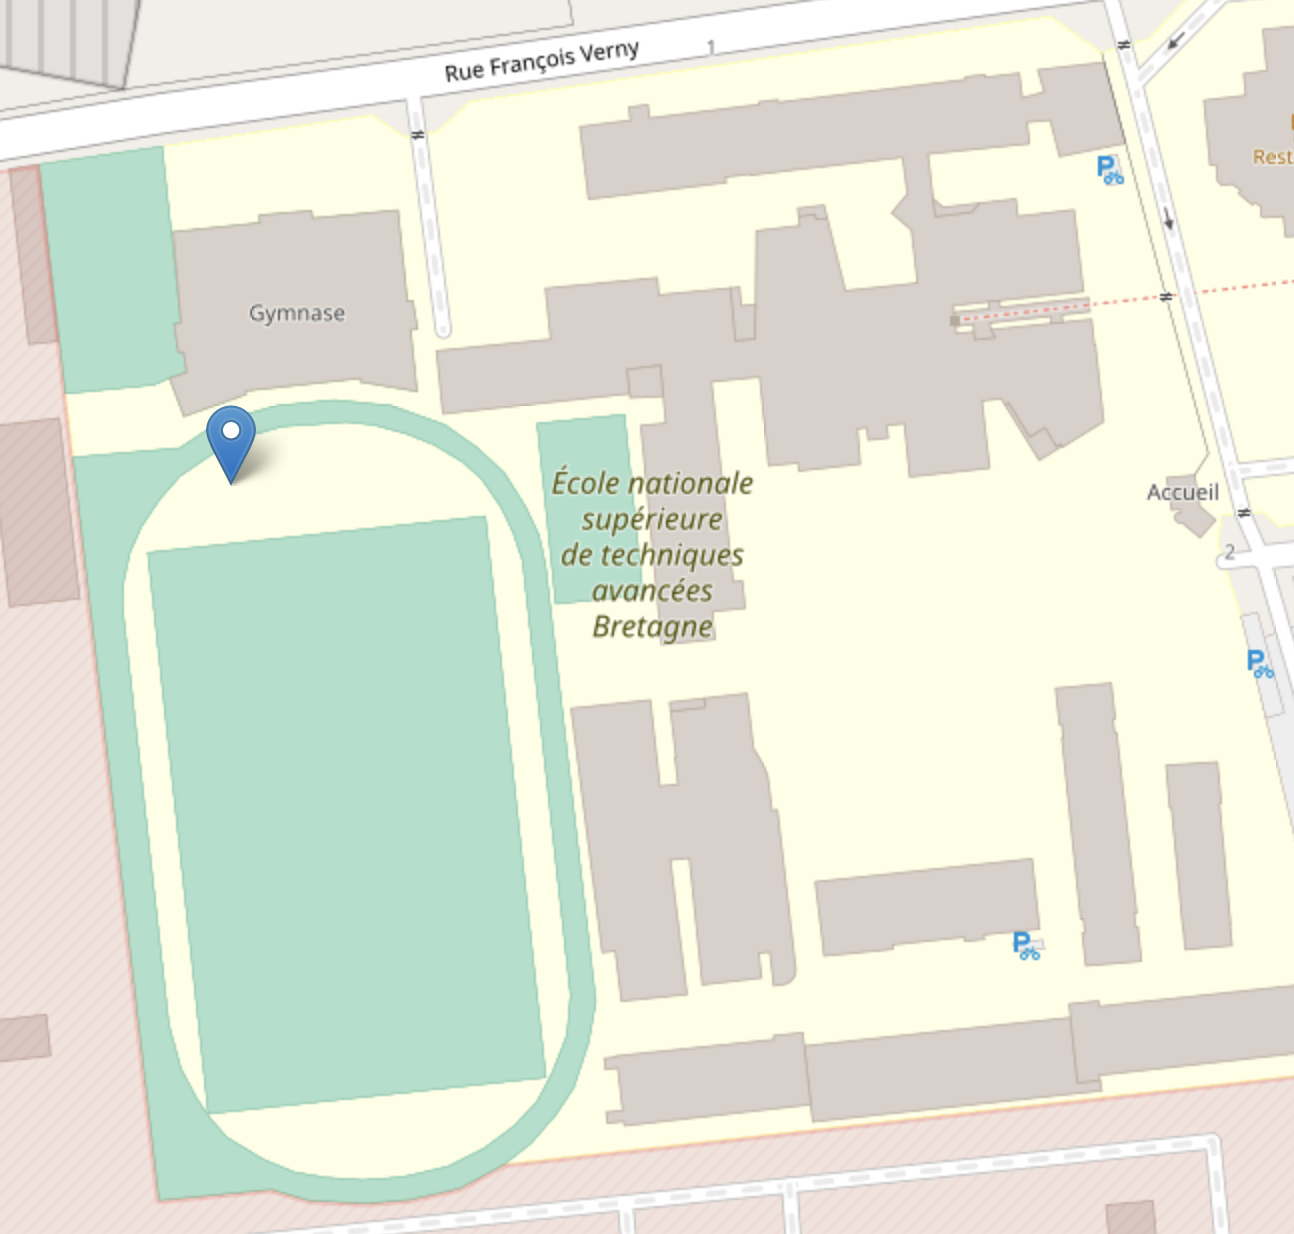
\includegraphics[width=.7\textwidth]{imgs/point_fixe}
          \caption{Position du point de référence}
          \label{fig:pt-fixe}
      \end{figure}

   \subsection{Études menées}\label{subsec:etudes-menees}
      Ces prises de mesures nous ont permis d'obtenir deux fichiers NMEA à exploiter, contenant entre autres les mesures successives de position de chaque récepteur.

      \begin{figure}[h]
          \centering
          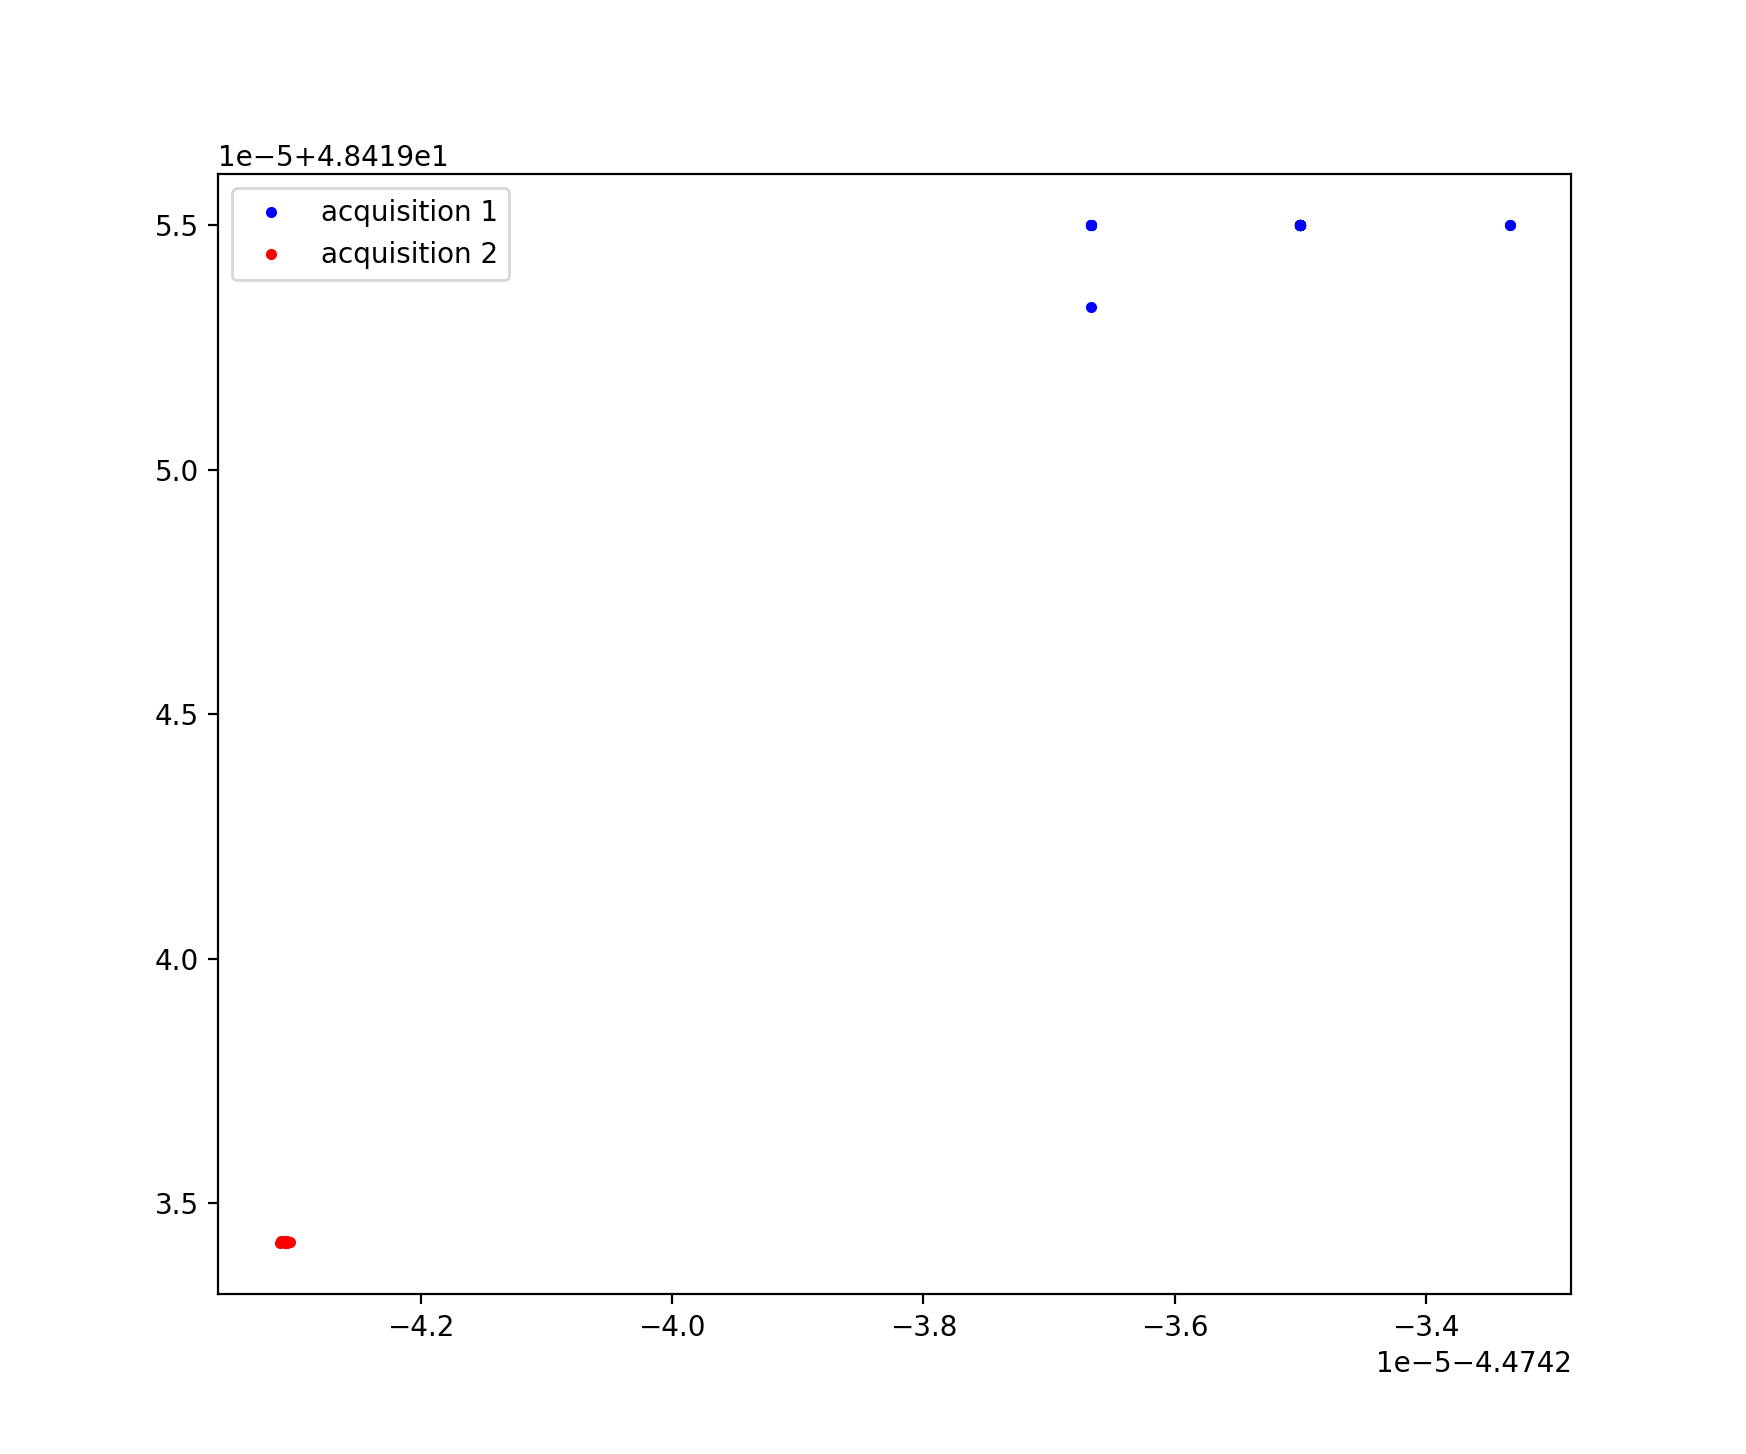
\includegraphics[width=.8\textwidth]{imgs/fidélité}
          \caption{Points mesurés par les récepteurs}
          \label{fig:fidel}
      \end{figure}

      \subsubsection{Étude de la fidélité}
         Une première étude que nous avons décidé de mener, étant donné l'allure des mesures prises est une étude statistique.
         Il nous a donc été possible de calculer, pour chaque acquisition, une coordonnée moyenne ainsi que des écarts-type, ayant tout naturellement mené vers l'estimation d'une incertitude statistique (type A), dont les résultats sont présentés dans le tableau placé en annexe.

         On peut entre autres remarquer une dispersion plus forte pour le récepteur le moins précis, ce qui est bien le résultat que nous attendions.

      \subsubsection{Étude de la justesse}
         Une seconde analyse menée a été une comparaison des positions moyennes aux coordonnées connues du point de référence, dont les résultats sont également présentés dans le tableau en annexe.

         Il est cependant possible de remarquer que le récepteur le moins précis a une précision mesurée de l'ordre du mètre, tandis que le récepteur le plus précis a une précision de l'ordre du millimètre.
